BootstrapはTwitterが生み出したオープンソースのフロントエンド開発のツールパッケージです。開発者にとっては、Bootstrapは素早いWebアプリケーション・プログラムの開発における最良のフロントエンドツールパッケージです。これはCSSとHTMLのセットで、最新のHTML5標準を使用しています。Web開発のモダンなバージョン、フォーム、ボタン、テーブル、ネットワークシステム等を提供します。


\begin{itemize}
  \item モジュール Bootstrapには豊富なWebモジュールが含まれています。これらのモジュールによって美しく、機能の揃ったページを作成することができます。これには以下のモジュールが含まれています: プルダウンメニュー、ボタンセット、ボタンプルダウンメニュー、ナビゲーション、ナビゲーションバー、パンくずリスト、ページング、ランキング、サムネイル、エラーダイアログ、プログレスバー、メディアオブジェクト等
  \item Javascriptプラグイン Bootstrapは13個のjQueryプラグインを備えています。これらのプラグインはBootstrapのモジュールに"生命"を与えます。これには以下が含まれます: モードダイアログ、ラベルページ、スクロールバー、ポップアップウィンドウ等
  \item カスタマイズしたフレームワークのコード BootstrapのすべてのCSS変数は修正できます。自分の好みに合わせてコードを切り取ることができます。
\end{itemize}


\begin{figure}[H]
   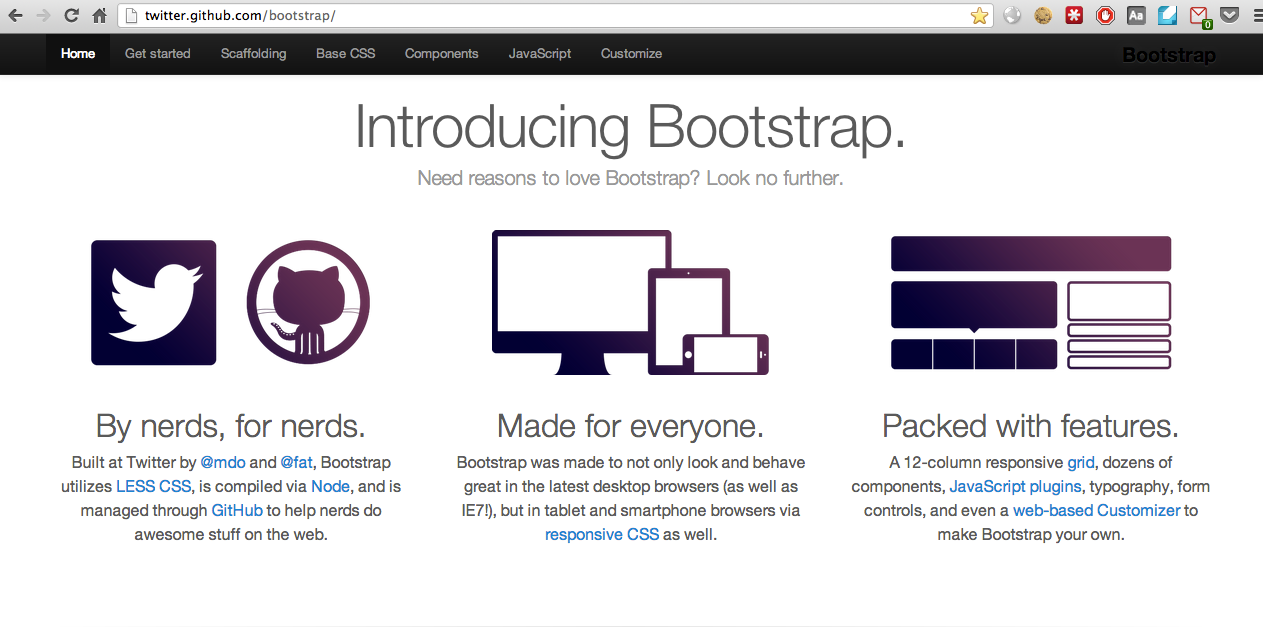
\includegraphics[width=14cm]{14.1.bootstrap.png}
   \label{図14.1}
   \caption{bootstrapサイト}
\end{figure}



次にbootstrapをbeegoフレームワークに集めることで、美しいサイトを作成することができます。

\begin{enumerate}
  \item まずダウンロードしたbootstrapディレクトリを我々のプロジェクトのディレクトリに展開します。以下のスクリーンショットのように名前をstaticとします。
\begin{figure}[H]
   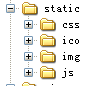
\includegraphics[width=5cm]{14.1.bootstrap2.png}
   \label{図14.2}
   \caption{プロジェクトにおける静的なファイルのディレクトリ構造}
\end{figure}
  \item beegoはデフォルトでStaticDirの値を設定しますので、あなたの静的なディレクトリがstaticであれば、追加する必要はありません:\\ StaticDir["/static"] = "static"
  \item テンプレートで以下のようなアドレスを使用すればOKです:
\begin{lstlisting}[numbers=none]
//cssファイル
<link href="/static/css/bootstrap.css" rel="stylesheet">

//jsファイル
<script src="/static/js/bootstrap-transition.js"></script>

//画像ファイル
<img src="/static/img/logo.png">
\end{lstlisting}
\end{enumerate}

上ではbootstrapをbeegoの中に実装しています。以下に示す図は実装後の効果図です:


\begin{figure}[H]
   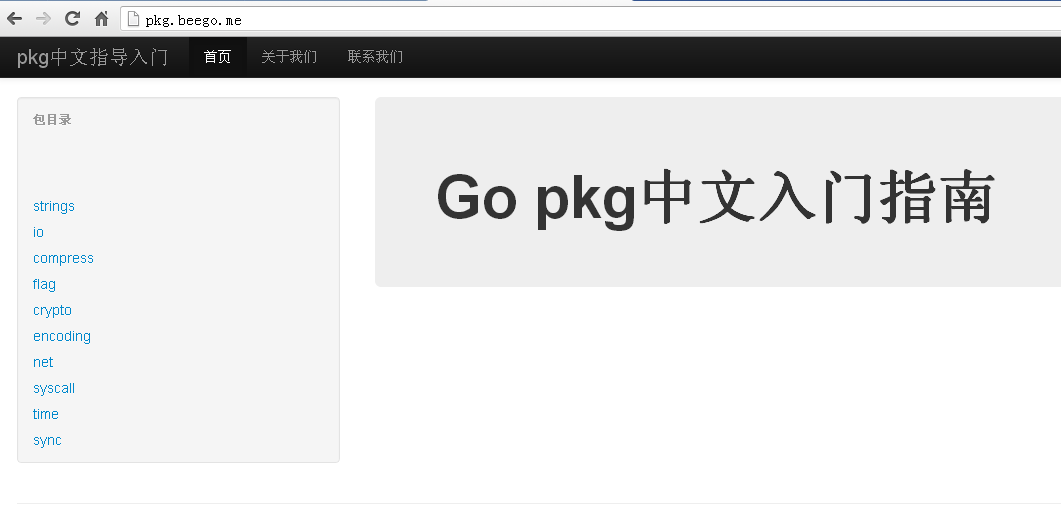
\includegraphics[width=14cm]{14.1.bootstrap3.png}
   \label{図14.3}
   \caption{bootstrapにもとづいて作成されたサイトのインターフェース}
\end{figure}


これらのテンプレートとフォーマットはbootstrapのオフィシャルが提供しているものです。ここではコードを再び貼り直すことはしません。みなさんはbootstrapのオフィシャルサイトでどのようにテンプレートを記述するか学んでください。
